\section{Misalignment Studies} \label{sec:misalign}

In order to protect both the active area of the SiPMs and the scintillator surface at the upstream end, the coupling distance between the two was required to be larger than zero.  Similarly, during assembly the scintillator paddles were also shimmed radially such that the top edge of the scintillator was level with the top edge of the active area of the SiPM thereby maximizing light collection.  In this section the coupling distance and vertical alignment, and its effect regarding light collection and time resolution, between a machined scintillator and SiPM are discussed.   

\subsection{Experimental Set-up} \label{sec:misalign_setup}

A custom fabricated test stand, discussed in Sec.~\ref{sec:fab_test}, and a polished scintillator machined to the nominal ST geometry were utilized for these studies.  The readout SiPM sat atop a Newport MT-XYZ (MT) compact dovetail XYZ linear translation stage\cite{newport_mt_xyz} with three fine adjustment screws consisting of 80 threads per inch.  Each knob for the three axes provides a translation of $318\ \mathrm{\mu m}$ per rotation.  For each location of the SiPM, the source and trigger PMT were located $\mathrm{24.5~cm}$ downstream from the readout end.

To study the effects of the various horizontal (translations along the $z-axis$) coupling distances, the relative position of the active area of the SiPM and the top edge of the scintillator paddle, or vertical (translations along the $y-ais$) alignment, was required to be known prior too.

Utilizing an Edmund Optics CMOS camera, and a reference ruler (seen in Fig. \ref{fig:sipm_va_optics}) the vertical alignment of the top edges of the SiPM and scintillator were measured with $\mathrm{0.025~mm}$ accuracy.
\begin{figure}[!htb]
	\centering
	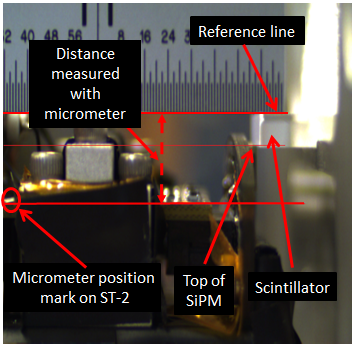
\includegraphics[width=1.0\columnwidth]{misalignment/figs/sipm_va_optics}
	\caption{Vertical alignment optics set-up.  The reference line corresponds to the top surface of the scintillator, while the micrometer position on the ST2 is clearly marked so that the absolute difference could be measured both optically and manually with a micrometer.}
	\label{fig:sipm_va_optics}
\end{figure}
A micrometer was utilized in order to cross check the optical measurements and to provide absolute measurements of fixed distances in the experimental set-up.  We have defined that at $y = 0$ the SiPM and scintillator are aligned vertically.  The coupling distance between the active area of the SiPM and scintillator ($z$) was set to a distance of $\mathrm{100\ \mu m}$ and monitored closely during the vertical alignment scan.

\subsection{Vertical Alignment of SiPM \& Scintillator}
\label{sec:misalign_vert}

To measure the time resolution at various vertical alignment configurations the scintillator remained fixed while the SiPM scanned across the upstream end of the scintillator. The SiPM was lowered to the minimum location governed by the range of the MT translation stage.  This distance was measured to be $y = \mathrm{-4~mm}$.  

``Coarse'' measurements were then taken at half turn intervals $(159\ \mathrm{\mu m})$ until the maximum height of the MT translation stage was reached which was approximately $y = +4\ \mathrm{mm}$.  In order to conduct ``precise'' measurements the SiPM was lowered to $y = \mathrm{-1~mm}$ and then the translation stage was moved in quarter turn intervals $(79.5\ \mathrm{\mu m})$ until it reached $y = \mathrm{+1~mm}$.  The results of these measurements can be seen in Fig. \ref{fig:sipm_va_coarse}.
\begin{figure}[!htb]
	\centering
	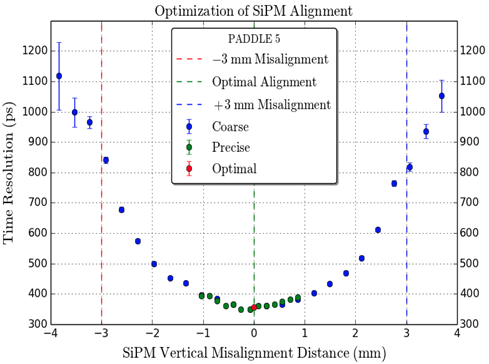
\includegraphics[width=1.0\columnwidth]{misalignment/figs/sipm_va_coarse_v2}
	\caption{Coarse vertical misalignment results.  The minimum time resolution obtained was approximately 350 ps which was expected.  Once the SiPM exceeded $y = \pm 3\ mm$ there is no active area of the SiPM coupled to the face of the scintillator.}
	\label{fig:sipm_va_coarse}
\end{figure}
For each distinct location of the SiPM, the distance traversed was verified by a manual measurement made with a micrometer with $25\ \mu m$ precision.

From the vertical misalignment studies it is clear that there is no significant variation of time resolution within a $\pm 300\ \mathrm{\mu m}$ range of the optimal alignment.  These results were also simulated in a manner similar to what was discussed in section \ref{sec:sim_mach} and the results are seen in Fig. \ref{fig:vertical_sim}.
\begin{figure}[!htb]
	\centering
	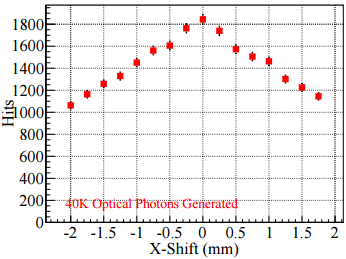
\includegraphics[width=1.0\columnwidth]{misalignment/figs/vertical_sim}
	\caption{Vertical alignment simulation studies \cite{puneet_sim_talk}.  It is important to note the x-axis corresponds to the y-axis as discussed with the experimental measurements.}
	\label{fig:vertical_sim}
\end{figure}
The GEANT4 simulations indicate that the acceptable range of vertical misalignment is approximately $\pm 250\ \mathrm{\mu m}$ \cite{puneet_sim_talk} which is consistent with what was measured on the bench.

\subsection{Coupling Distance of SiPM \& Scintillator}

With the vertical alignment between the scintillator and SiPM optimized, the effects of varying the coupling distance were also studied.  Using an identical set-up as was described in section \ref{sec:misalign_vert} the coupling distance, and resulting time resolutions, were measured at various locations with three distances shown in Fig. \ref{fig:sipm_coupling_optics}.  
\begin{figure}[!htb]
	\centering
	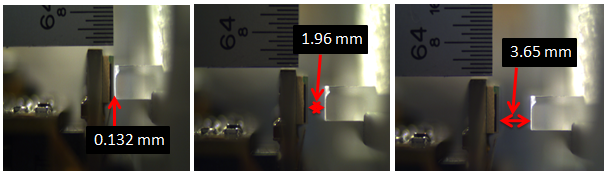
\includegraphics[width=1.0\columnwidth]{misalignment/figs/sipm_coupling_optics}
	\caption{Various coupling distances as measured with the CMOS camera.  The high degree of precision is clearly visible.}
	\label{fig:sipm_coupling_optics}
\end{figure}
While the coupling distance was varied, the vertical alignment was kept constant at the optimal location and was monitored both optically and manually with a micrometer.

The SiPM was moved \textit{via} the MT translation stage along the $z-axis$.  We defined $z = 0$ to be the instance when the active area of the SiPM was flush against the face of the machined scintillator paddle.  In the coupling region $z < 1\ \mathrm{mm}$ the SiPM was receded from the face of the SiPM in 1/4 turn intervals ($79.5\ \mathrm{\mu m}$).  For $\mathrm{1\ mm < z < 2\ mm}$, the SiPM was receded from the face of the SiPM in 1/2 turn intervals ($159\ \mathrm{\mu m}$), and for $\mathrm{2\ mm < z < 4\ mm}$ data were collected in 1 turn intervals ($\mathrm{318\ \mu m}$) with the results being illustrated in Fig. \ref{fig:sipm_coupling_coarse}.
\begin{figure}[!htb]
	\centering
	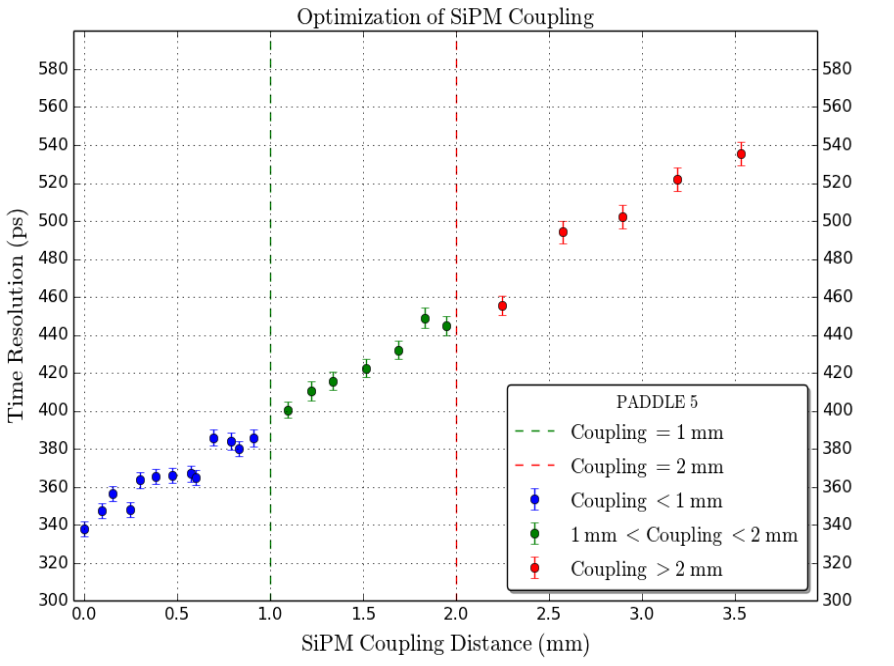
\includegraphics[width=1.0\columnwidth]{misalignment/figs/sipm_coupling_coarse}
	\caption{Coarse coupling distance studies.  It is useful to note that at a coupling distance of $\mathrm{251\ \mu m}$ the time resolution was identical to what was measured in Fig. \ref{fig:sipm_va_fine} while conducting the vertical alignment studies.}
	\label{fig:sipm_coupling_coarse}
\end{figure}

It is clear from the data the optimal coupling range was $\mathrm{50\ \mu m < z < 350\ \mu m}$ and there was no significant reduction in time resolution performance over a $\mathrm{0\ \mu m < z < 600\ \mu m}$ range.  Similarly, the simulation results seen in Fig.~\ref{fig:spacing_sim} also indicate that there is no significant reduction in light collection in the $\mathrm{0\ \mu m < z < 600\ \mu m}$ range \cite{puneet_sim_talk}.
\begin{figure}[!htb]
	\centering
	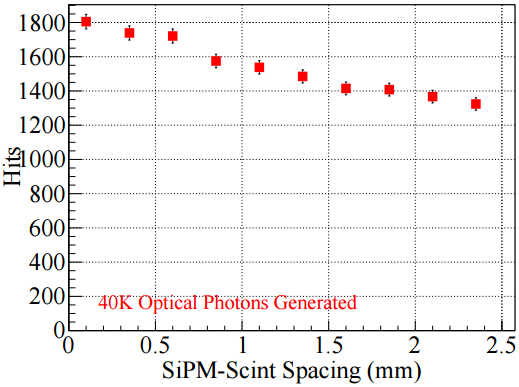
\includegraphics[width=1.0\columnwidth]{misalignment/figs/spacing_sim}
	\caption{Coupling distance simulations. Simulations indicated that the optimal coupling distance is in the $50\ \mu m < z < 350\ \mu m$ range.}
	\label{fig:spacing_sim}
\end{figure}


